%%%%%%%%%%%%%%%%%%%%%%%%%%%%%%%%%%%%%%%%%
% Stylish Article
% LaTeX Template
% Version 2.2 (2020-10-22)
%
% This template has been downloaded from:
% http://www.LaTeXTemplates.com
%
% Original author:
% Mathias Legrand (legrand.mathias@gmail.com) 
% With extensive modifications by:
% Vel (vel@latextemplates.com)
%
% License:
% CC BY-NC-SA 3.0 (http://creativecommons.org/licenses/by-nc-sa/3.0/)
%
%%%%%%%%%%%%%%%%%%%%%%%%%%%%%%%%%%%%%%%%%

%----------------------------------------------------------------------------------------
%	PACKAGES AND OTHER DOCUMENT CONFIGURATIONS
%----------------------------------------------------------------------------------------

\documentclass[fleqn,10pt]{SelfArx} % Document font size and equations flushed left

\usepackage[english]{babel} % Specify a different language here - english by default

\usepackage{subcaption}
\usepackage{svg}
\usepackage{url}
\setlength{\headheight}{20.96901pt}

\usepackage{lipsum} % Required to insert dummy text. To be removed otherwise
\usepackage{ragged2e} % for justifying

%----------------------------------------------------------------------------------------
%	COLUMNS
%----------------------------------------------------------------------------------------

\setlength{\columnsep}{0.55cm} % Distance between the two columns of text
\setlength{\fboxrule}{0.75pt} % Width of the border around the abstract

%----------------------------------------------------------------------------------------
%	COLORS
%----------------------------------------------------------------------------------------

\definecolor{color1}{RGB}{0,0,90} % Color of the article title and sections
\definecolor{color2}{RGB}{0,20,20} % Color of the boxes behind the abstract and headings

%----------------------------------------------------------------------------------------
%	HYPERLINKS
%----------------------------------------------------------------------------------------

\usepackage{hyperref} % Required for hyperlinks

\hypersetup{
	hidelinks,
	colorlinks,
	breaklinks=true,
	urlcolor=color2,
	citecolor=color1,
	linkcolor=color1,
	bookmarksopen=false,
	pdftitle={Title},
	pdfauthor={Author},
}

%----------------------------------------------------------------------------------------
%	ARTICLE INFORMATION
%----------------------------------------------------------------------------------------

\JournalInfo{Neuro 120, Final Project, May 5, 2023} % Journal information
\Archive{Professor Kristina Penikis} % Additional notes (e.g. copyright, DOI, review/research article)

\PaperTitle{Constructing an EEG-Based Music Emotion Recognition Model with either Deep or Convolutional Neural Networks} % Article title

\Authors{Ricardo Marrero-Alattar\textsuperscript{1}, Matthew Vu\textsuperscript{2}} % Authors
\affiliation{\textsuperscript{1}\textit{Department of Neuroscience, Harvard University, Cambridge, United States}} % Author affiliation
\affiliation{\textsuperscript{2}\textit{Department of Neuroscience, Harvard University, Cambridge, United States}} % Author affiliation

\Keywords{} % Keywords - if you don't want any simply remove all the text between the curly brackets
\newcommand{\keywordname}{Keywords} % Defines the keywords heading name

%----------------------------------------------------------------------------------------
%	ABSTRACT
%----------------------------------------------------------------------------------------

\Abstract{This study investigates the efficacy of deep neural networks (DNNs) and convolutional neural networks (CNNs) in recognizing emotions from electroencephalography (EEG) data induced by musical stimuli. The aim is to explore how different neural network architectures and data representations—raw EEG voltage-time data and EEG-derived spectrograms—impact the accuracy of music emotion recognition (MER). Using the Music Listening-Genre EEG dataset (MUSIN-G), which includes EEG recordings from 20 non-musician participants exposed to a variety of musical genres, we processed the data to generate both raw and spectrogram formats. The neural models were then trained to classify emotional responses into four categories based on the participants' ratings of familiarity and enjoyment. Our findings reveal that while both DNNs and CNNs demonstrated potential in decoding emotional cues from EEG data, the performance was generally near or below random chance, indicating significant challenges in model training and data quality. The DNNs, in particular, tended to predict a single class irrespective of the input, suggesting overfitting or inadequate feature extraction capabilities. This research underscores the complexities of applying neural networks to EEG-based emotion recognition and highlights the need for refined data processing techniques and model parameters to enhance future implementations in humanizing artificial intelligence through emotional intelligence.}

%----------------------------------------------------------------------------------------

\begin{document}

\maketitle % Output the title and abstract box
\tableofcontents % Output the contents section
\thispagestyle{empty} % Removes page numbering from the first page

%----------------------------------------------------------------------------------------
%	ARTICLE CONTENTS
%----------------------------------------------------------------------------------------

\section*{Introduction} % The \section*{} command stops section numbering

\addcontentsline{toc}{section}{Introduction} % Adds this section to the table of contents
 
Music emotion recognition (MER) is the study of how to measure emotionally-induced changes in the brain following a musical stimulus (Cui et.al., 2022). As the intersection between music information retrieval (MIR) – i.e. the study of how the brain extracts information from music– and emotion recognition (ER), MER is useful because it can elucidate how music affects the brain while also contributing to the development of an automated emotion recognition algorithm that standardizes emotional intelligence, a crucial node in humanizing AI (Picard, 2003). Experiments looking at the neurobiological basis of ER are centered around electroencephalography (EEG), a method of recording spontaneous electrical (and thus neural) activity in the brain, due to its accessibility and high temporal resolution (Alarcão \& Fonseca, 2019). The latter is especially useful when studying MER, as recent studies using EEG show that not only do musical differences strongly correlate with changes in neural activity, but that MER is a rapidly occurring process (Vuilleumier and Trost, 2015). Furthermore EEG limits the probability that bodily responses to music are missed– a common problem in former methods of MER measurement– and it is preferred over functional magnetic resonance imaging (fMRI) due to the latter’s lack of temporal resolution and high background noise tainting the intended stimulus (Cui et.al., 2022). Given these reasons, it is unsurprising that over 100 studies have found consistent results in the inferred emotional response to different styles of music, and music therapy highlighting both the accuracy and potential for EEG-MER studies to flourish. 

MER has grown in popularity over the past decade (He \& Ferguson, 2020) because the advent of convolutional neural networks (CNNs) and deep neural networks (DNNs) has propelled the field by replacing traditional machine learning (ML) methods to develop stronger and more accurate models (Louro et.al., 2024; Jia, 2022). Other methods, such as support vector machine (SVM), K-nearest neighbor (KNN), and Random Forest (RF) have been proposed, but they do not compare to these two neural networks because they cannot (yet) extract deeper emotional features (Qiao, 2024). Differences in the capabilities of DNNs and CNNS have been explored in general emotion recognition, with most research showing that each has their own comparable advantages; for example, in text-based emotion recognition, DNNs exhibit resilience and flexibility in disentangling complicated relationships while CNNs capture local characteristics and spatial hierarchies better (Jadon \& Kumar, 2023). On the MIR side, scientists have shown that both CNNs and DNNs can perform at remarkably comparable accuracies (92\% vs 90\%) in music emotion \textit{classification} tasks (Kamala \& Hassani, 2022), but the challenge remains as to whether this parallelism in efficiency translates to \textit{recognition} models. While hybrid models have been used before (Jia, 2022), the key advantages and disadvantages of using DNNs vs CNNs in MER models have yet to be fully explored.

Given that both types of neural networks require pure, accurate, and meaningful data, EEG-based studies can choose between two approaches to the data processing step. The first is to simply use the raw data, itself an oscillating curve representing the change in voltage over time. One of the main benefits of using this raw data is that artifacts– which can appear easily in EEG studies through blinks or other involuntary human tendencies, can be more easily corrected. Separately, using the raw data preserves the signal amplitude, complex waveforms, and other potentially useful variables in the data. In contrast, spectrograms lose the precise timing of certain neural events, instead condensing the time axis into windows such that it displays frequency over time. This loss is compensated by the provision of variations in neural activity across different frequency bands (e.g. alpha, gamma, etc.). Whether it is unto a spectrogram or another more complicated method, this process of splitting the raw data into frequency bands makes the data more specific and has been shown to be the most effective way to determine MER from EEG signals (Shen et.al., 2021, Ghodousi et.al., 2022; Cui, Li, \& Touyama, 2023).

That said, the creators and users of the DEAP dataset (Koelstra et.al., 2012) have already begun expanding to new methods to increase the range of determinable knowledge from the data, including analyzing the interrelationships between electrodes (Cui, Li, \& Touyama, 2023) and a graphical view of neural relationships across the brain (Ding et al., 2023). However, it is still not fully understood what kinds of neural networks (and with what kind of data processing) would yield the best results for general recognition accuracy. Therefore, this paper seeks to contribute to the foundation of this field of study by answering the following research questions:

\begin{enumerate}
    \item Will raw voltage vs time data outperform a spectrogram as training inputs for an MER model?
    \item How does changing the type of neural network (given either type of training input) affect the accuracy of the model?
\end{enumerate}

%------------------------------------------------

\section{Methods}

This section explains the methods used for this experiment. 
\begin{figure}
    \centering
    \includegraphics[width=1\linewidth]{1-s2.0-S235234092200868X-gr1.jpg}
    \caption{Behavioral Data (Miyapuram, 2022)}
    \label{fig:data_dist}
\end{figure}

\flushleft\subsection{The MUSIN-G Dataset}
\justifying
The Music Listening-Genre EEG dataset (MUSIN-G)  dataset was made publicly available on OpenNeuro (Miyapuram et.al., 2022). The dataset had 20 non-musician participants from India listen to a genre-unique set of 12 songs with a 1SD average duration (in seconds) of 119 ± 2.475 (±2.08).  Participants closed their eyes and listened to the full duration of the song (start and end indicated by 1 \& 2 beeps respectively), and then rated the song on a linear 1-5 scale for both the song’s familiarity and enjoyment. The figure adjacent plots the results, demonstrating how each participant (blue dot) rated each song (X-axis) on how enjoyable (Y1 axis) or familiar (Y2 axis) the music felt (Miyapuram et.al., 2022). Throughout the experiment, participants wore a high-density 128-electrode EEG cap and had their neural activity recorded.
\begin{figure}
    \centering
    \caption{Enjoyment Ratings Histogram}
    \includegraphics[width=1\linewidth]{histogram enjoyment.png}
    \label{fig:enjoy_hist}
\end{figure}
\begin{figure}
    \centering
    \includegraphics[width=1\linewidth]{histogram frequency.png}
    \caption{Familiarity Ratings Histogram}
    \label{fig:famil_hist}
\end{figure}
\subsection{Data Processing}

\begin{figure*}
    \centering
    \begin{subfigure}[b]{0.45\linewidth} % Adjust the width of the subfigure, here it is 50% of the line width
        \centering
        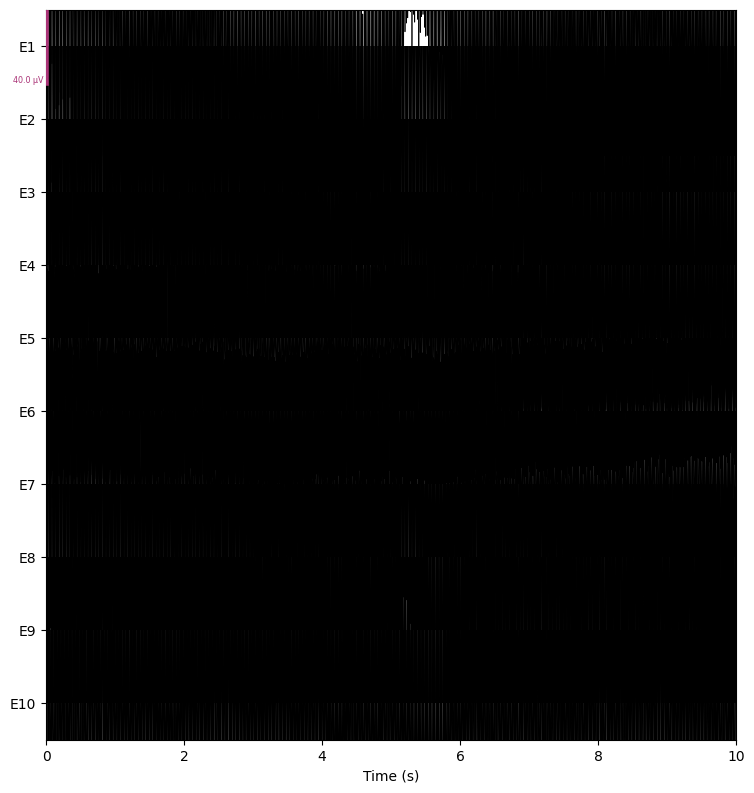
\includegraphics[width=\linewidth]{Figures/raw_VT.png}
        \caption{\textbf{Before preprocessing:} Voltage vs. time for subject 5 listening to song 11}
        \label{fig:raw_VT}
    \end{subfigure}%
    % add more subfigures here if you have more images
    \begin{subfigure}[b]{0.45\linewidth} % Another subfigure
        \centering
        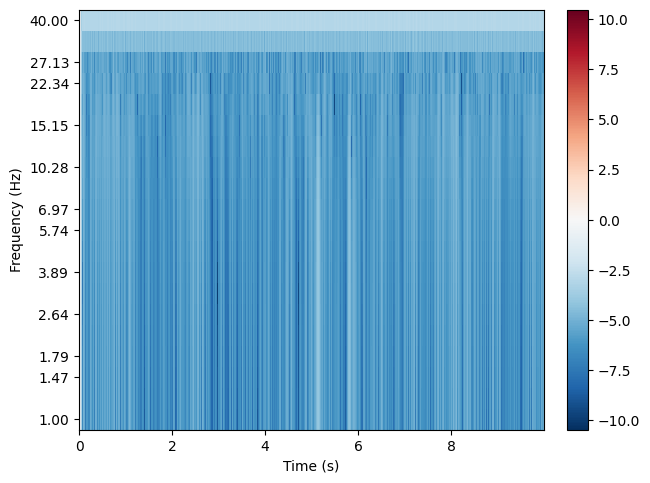
\includegraphics[width=\linewidth]{Figures/raw_spec.png} % Adjust path accordingly
        \caption{\textbf{Before preprocessing:} Channel 1 spectrogram for subject 5 listening to song 11}
        \label{fig:raw_spec}
    \end{subfigure}
    \begin{subfigure}[b]{0.45\linewidth} % Another subfigure
        \centering
        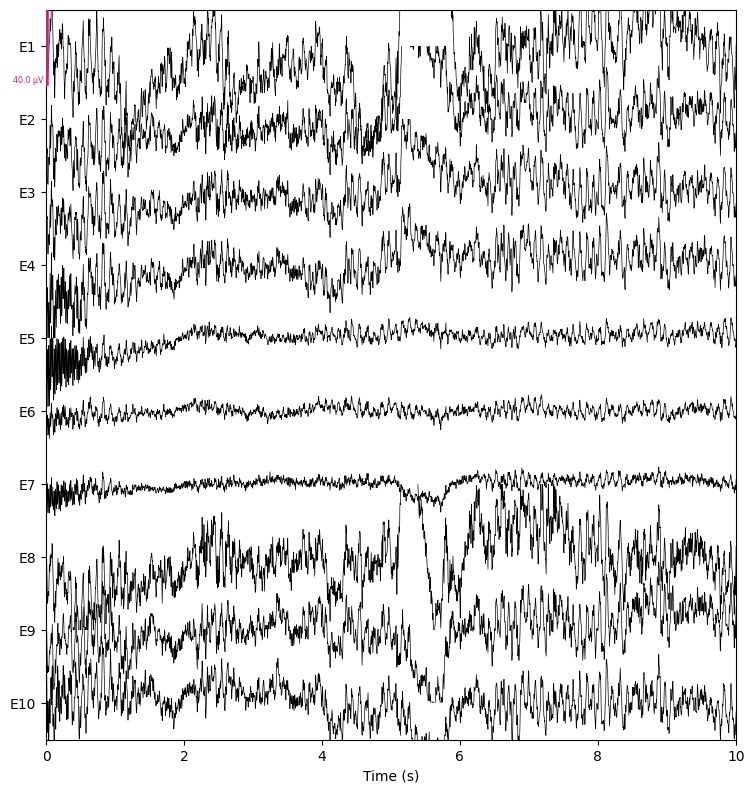
\includegraphics[width=\linewidth]{Figures/pre_VT.png} % Adjust path accordingly
        \caption{\textbf{After preprocessing:} Voltage vs. time for subject 5 listening to song 11}
        \label{fig:pre_VT}
    \end{subfigure}
    \begin{subfigure}[b]{0.45\linewidth} % Another subfigure
        \centering
        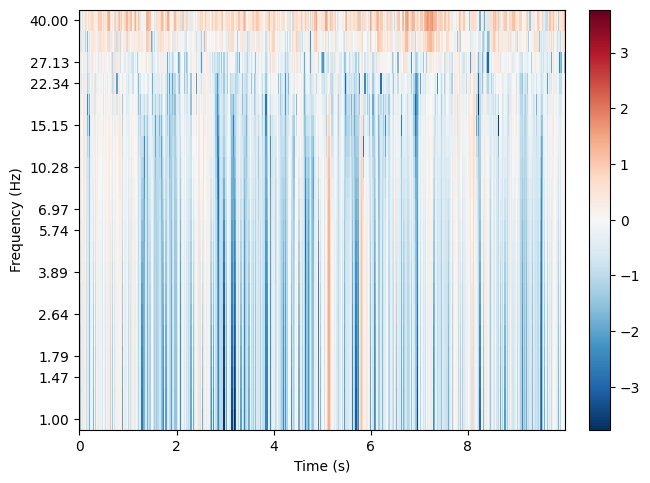
\includegraphics[width=\linewidth]{Figures/pre_spec.png} % Adjust path accordingly
        \caption{\textbf{After preprocessing:} Channel 1 spectrogram for subject 5 listening to song 11}
        \label{fig:pre_spec}
    \end{subfigure}
    \caption{Example data from the MUSIN-G dataset before and after our preprocessing steps}
    \label{fig:data_processing}
\end{figure*}

The steps to convert the data into a readable format for the neural networks were closely based on former experiments of similar nature (Qian et.al., 2022, Chaddad et.al., 2023; Pandey et.al., 2023). Using MNE-Python (minimum norm estimation) software, which is an algorithm that localizes EEG sources (Newman, MNE-Python), the following steps were performed:

    \begin{enumerate}
        \item Applied a high-pass filter at 0.2 Hz to correct for slow drifts and baseline fluctuations, which can arise from environmental noise or physiological changes
        \item Removed the 50 Hz line noise,  which typically arises from the local power supply
        \item Downsampled the signal to 256 Hz to reduce the sampling rate while preserving the critical frequency content necessary for the neural networks
        \item Calculated the power spectral density (PSD) of the signal via Welch’s method, which determines which frequency components of the signal have larger variations
        \item Set the threshold for a good vs a bad EEG channel to be 3 standard deviations from the mean PSD across the frequency axis, with bad referring to a channel with unusually high spectral power relative to the mean (which may indicate noise or artifacts)
        \item Interpolated the bad channels (i.e. estimated their values based on surrounding information) to reduce any additional noise 
        \item Performed Independent Component Analysis (ICA) on the data to remove artifacts and isolate the neural activity
        \item Re-referenced the data to the average, i.e. subtracted the average signal from each channel’s signal to remove common noise between the channels.
    \end{enumerate}
    
Undergoing these preprocessing steps allowed for the data to focus purely on dynamic neural activity.

\subsection{Preparing the Data to Feed Into the Neural Networks}

\paragraph{Data Preprocessing and Tensor Transformation}
Prior to the application of neural network models, the EEG data underwent a rigorous preprocessing routine. Initially, the data was organized into tensors to serve as input for convolutional neural networks (CNNs) and densely connected neural networks (DNNs).

For CNN inputs, the EEG data was restructured into a tensor format comprising 129 channels and 1,250 time bins, effectively representing 5 seconds of EEG activity given the sampling rate of 250 Hz. This transformation preserved the temporal and spatial dimensions of the data, crucial for capturing dynamic neural interactions over time.

Conversely, for inputs to DNNs, the data was flattened, transforming the tensor into a two-dimensional array where spatial and temporal information was concatenated into a single vector. This format is particularly suited for models that do not inherently process the data in its original three-dimensional form.

\paragraph{Spectrogram Construction}
For spectrogram-based inputs, the frequency domain was discretized into 20 bins ranging from 1 to 40 Hz. To construct the spectrograms, we applied Morlet wavelets with eight cycles per frequency, employing a fast Fourier transform for the time-frequency analysis. This process resulted in an initial spectrogram tensor shape of 129 channels by 20 frequency bins by 84 time bins, each time bin corresponding to approximately 1 second of EEG data.

To optimize the tensor for neural network processing and reduce computational demands, we averaged the spectrogram data across adjacent time bins. This averaging reduced the time resolution, compressing the original 84 time bins into 42, yielding a reshaped tensor of dimensions (129, 20, 42). For model compatibility, we further flattened the frequency and time dimensions, resulting in a final tensor shape of (129, 840). This transformation was essential to accommodate the limited computational resources available, as processing larger spectrogram windows would significantly increase both computational time and resource consumption during model training and backpropagation.

Each method of data transformation was selected to best utilize the architectural strengths of the corresponding neural network models, ensuring efficient processing while maintaining the integrity and resolution necessary for robust EEG analysis.

For our labels, we binned the enjoyment and familiarity ratings into 4 different categories:
\begin{enumerate}
    \item High enjoyment and high familiarity
    \item High enjoyment and low familiarity
    \item Low enjoyment and high familiarity
    \item Low enjoyment and low familiarity
\end{enumerate}

where high was any rating 3 or above, and low was any rating 2 or below.

\subsection{Constructing the Neural Networks}

This section will discuss how the two networks were built. 

\paragraph{Deep Neural Network} 

The  deep neural network with raw data input was constructed with 512 nodes forming the first layer from the input (size 129 electrodes by 1250 time bins), followed by a second layer of 256 nodes and a third layer of 128 nodes. This third layer connected to the 4 classes at the end of the network. Three layers is generally considered the maximum number of layers before the jumps in performance ability dwindle (Carle, 2002). The input tensor was flattened such that it matched the expected input dimensions of the first fully connected layer, which was a necessary step given that the input tensor had several dimensions (batch size, channels, and data points). A rectified linear unit (ReLU) function was applied to the outputs of each layer such that any negative values would be neutralized and the positive activations were isolated. In doing so, the model effectively removed the role of inhibitory neurons in the system. After transforming the input images into tensors, the data loaders were constructed and given a sampling strategy specifically to target the imbalance in the amount of data in each class. Importantly, the output layer was not given a ReLU function because instead it would be the site of  then passed through a Cross Entropy Loss function for classification (de Boer, 2005). Lastly, an Adam optimizer (an extension of the gradient descent) with a learning rate of 0.0001 and a weight decay of 0.00001 was applied to correct bias and minimize overfitting. This optimizer was chosen because Adam optimizers typically converge faster than gradient descent (Leo, 2024).

The deep neural network with the spectrogram input was built to similarly to the raw-input DNN. However, there were several notable differences:
\begin{enumerate}
\item There were only two hidden layers instead of three, sizes 512 and 256 neurons.
\item The input had a 2 dimensional shape (batch size and number of features)
\item The total loaded input size was 108360 to match the flattened input size
\end{enumerate}

\paragraph{Convolutional Neural Network} 
The convolutional neural network with the raw-data input was constructed such that the first convolutional layer had 16 filters at a (3, 40) kernel size with (1, 20) padding. After batch normalizing, the second convolutional layer had 32 filters at a (3,25) kernel size with (1,12) padding. The third convolutional layer had 64 filters with a (3, 10) kernel size and (1,5) padding. After moving through three convolutional layers, max pooling is applied, where the first dimension is halved and the second dimension is quartered, hence reducing   the input feature map into windows of size (2,4). To prevent overfitting, two dropout layers of size 0.25 and 0.5 sequentially were applied. 100 features were mapped onto the classes with 19456 input points (64 channels by $17\times20$ area of the last feature map). 
From this point forward, the process was analogous to the deep neural networks. The images were transposed into tensor format, and the network was optimized using a Cross Entropy Loss function and an Adam optimizer with the same parameters.

The convolutional neural network with the spectrogram input was built  similarly to the raw-input CNN. However, the main difference was that the first convolutional layer had a (3,10) kernel size and a (1,5) padding, both of which were kept constant. In addition, the input size to the dense layer was much larger (430080 data points).

\begin{figure*}
    \centering
    \begin{subfigure}{\linewidth}
        \centering
        \includesvg[width=0.7\linewidth]{Figures/CNN_spec.svg}
        \caption{CNN architecture for the spectrogram data}
        \label{fig:CNN_spec_model}
    \end{subfigure}

    \begin{subfigure}{\linewidth}
        \centering
        \includesvg[width=0.7\linewidth]{Figures/CNN_VT.svg}
        \caption{CNN architecture for the voltage vs. time data}
        \label{fig:CNN_VT_model}
    \end{subfigure}

    \caption{Our proposed CNN model architectures}
    \label{fig:CNN_models}
\end{figure*}

\begin{figure*}
    \centering
    \begin{subfigure}{0.45\linewidth}
        \centering
        \includesvg[width=\linewidth]{Figures/MLP_spec.svg}
        \caption{DNN architecture for the spectrogram data}
        \label{fig:MLP_spec_model}
    \end{subfigure}
    \hfill % This adds optional horizontal spacing between the figures
    \begin{subfigure}{0.45\linewidth}
        \centering
        \includesvg[width=\linewidth]{Figures/MLP_VT.svg}
        \caption{DNN architecture for the voltage vs. time data}
        \label{fig:MLP_VT_model}
    \end{subfigure}

    \caption{Our proposed DNN model architectures}
    \label{fig:DNN_models}
\end{figure*}

%------------------------------------------------

\section{Results }
The general results were that the neural networks were incapable of accurately classifying the testing data. For the CNN trained on the spectrogram data, the accuracy lingered around 30\% for all 4 epochs of training, with a very variable validation accuracy, ranging from $\sim$20\% to $\sim$33\% (no better than random chance because we only have 4 classes). While the loss over epochs shot down to near 0 by the first epoch, it is clear in the confusion matrices that the network was exclusively guessing Low-Enjoyment Low-Familiarity for every data input. In contrast, the CNN trained on the raw data mostly guessed High-Enjoyment Low-Frequency for every data input. Optimistically, the accuracy range peaked at $\sim$55\%, but the validation accuracy maxed out to $\sim$35\%, mostly invalidating the results. This CNN  was the only one that showed traces of multiple classification categories (in this case in the Low-Enjoyment Low-Familiarity category). Underwhelmingly, both DNN networks lingered around random chance odds for classification each, presenting the same problem as the spectrogram CNN but exclusively guessing High-Enjoyment Low-Familiarity. 

These results, although disappointing, were not surprise-inducing as the networks, pre-processing, and spectrogram designs all needed to be simplified to stay on track of time and within computing resource limits. 


\begin{figure*}
    \centering
    \begin{subfigure}[b]{0.35\linewidth} % Adjust the width of the subfigure, here it is 50% of the line width
        \centering
        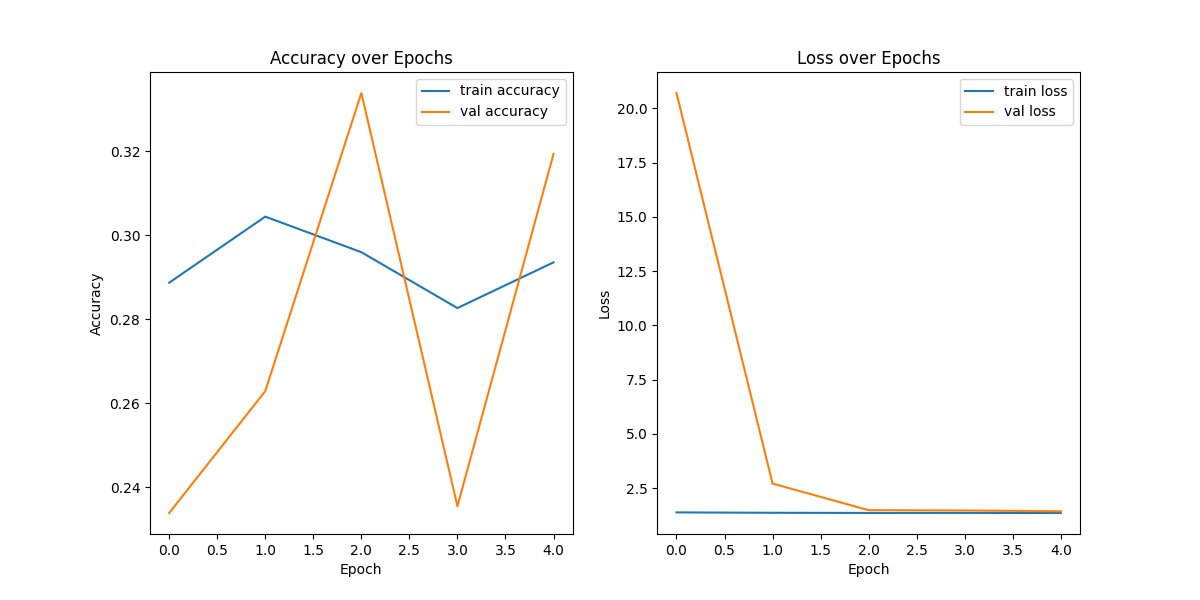
\includegraphics[width=\linewidth]{Figures/CNN_spec_loss_plot.png}
        \caption{Learning plots for the CNN trained on the spectrogram data}
        \label{fig:CNN_spec_loss_plot}
    \end{subfigure}%
    % add more subfigures here if you have more images
    \begin{subfigure}[b]{0.35\linewidth} % Another subfigure
        \centering
        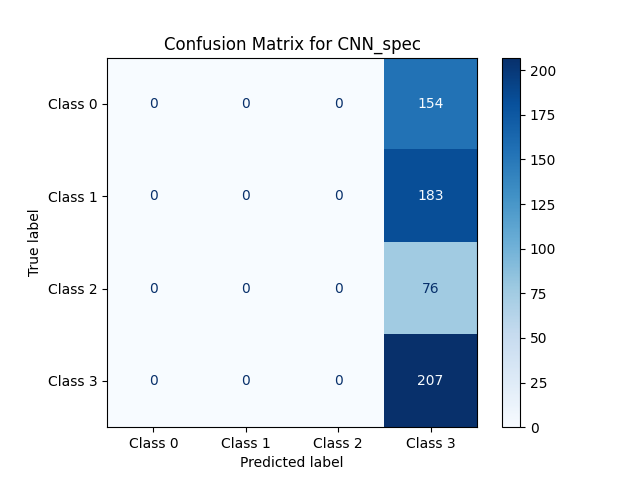
\includegraphics[width=\linewidth]{Figures/CNN_spec_confusion_mat.png} % Adjust path accordingly
        \caption{Confusion matrix for the CNN trained on the spectrogram data}
        \label{fig:CNN_spec_confusion_mat}
    \end{subfigure}
    \begin{subfigure}[b]{0.33\linewidth} % Another subfigure
        \centering
        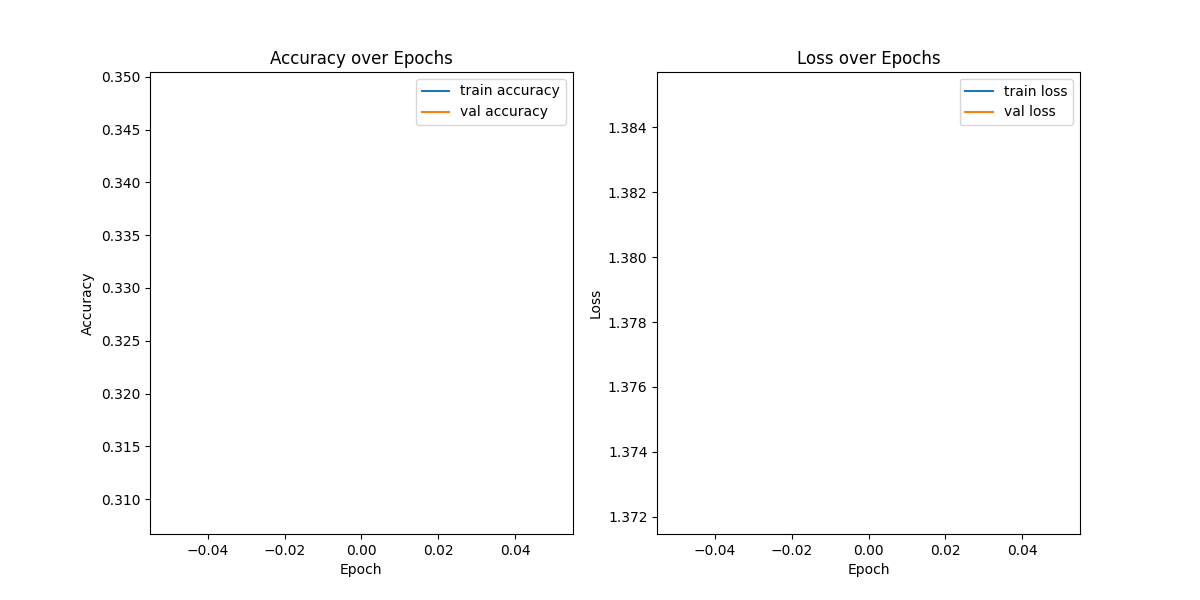
\includegraphics[width=\linewidth]{Figures/CNN_VT_loss_plot.png} % Adjust path accordingly
        \caption{Learning plots for the CNN trained on the voltage vs. time data}
        \label{fig:CNN_VT_loss_plot.png}
    \end{subfigure}
    \begin{subfigure}[b]{0.33\linewidth} % Another subfigure
        \centering
        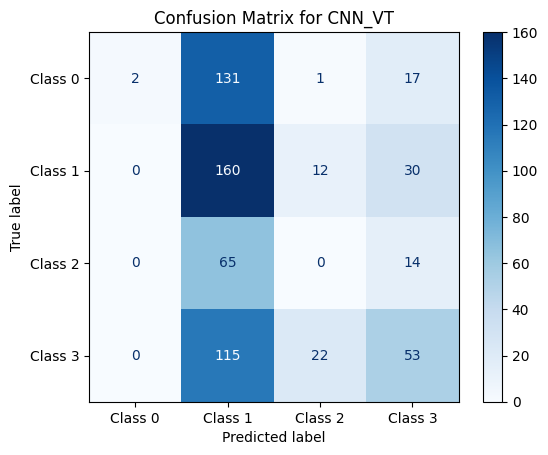
\includegraphics[width=\linewidth]{Figures/CNN_VT_confusion_mat.png} % Adjust path accordingly
        \caption{Confusion matrix for the CNN trained on the voltage vs. time data}
        \label{fig:CNN_VT_confusion_mat.png}
    \end{subfigure}
    \begin{subfigure}[b]{0.35\linewidth} % Another subfigure
        \centering
        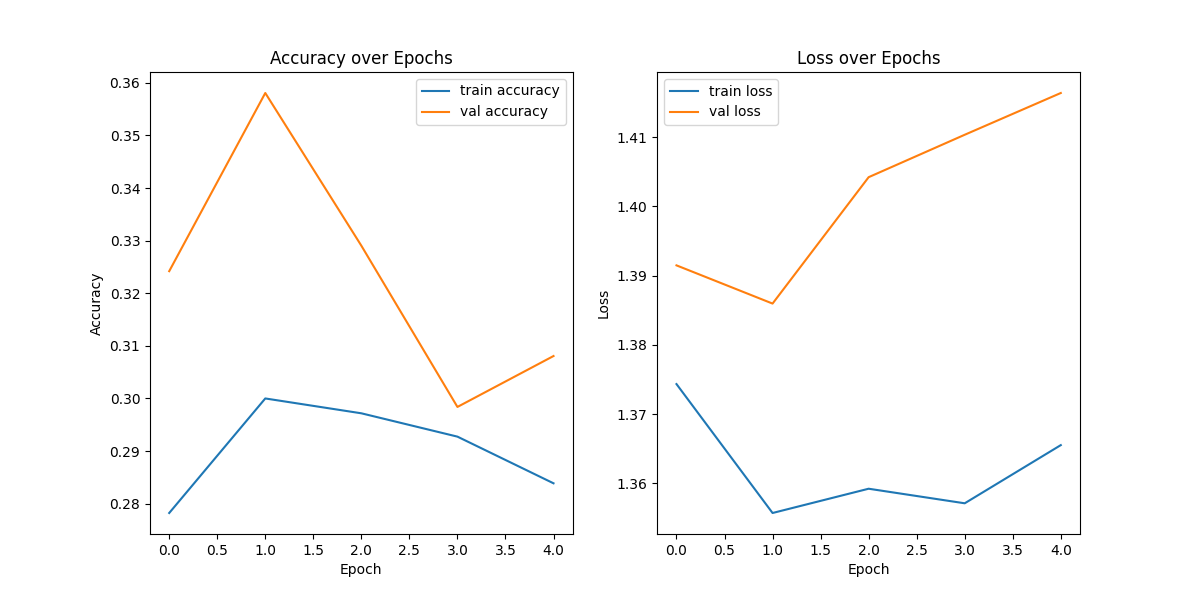
\includegraphics[width=\linewidth]{Figures/MLP_spec_loss_plot.png} % Adjust path accordingly
        \caption{Learning plots for the DNN trained on the spectrogram data}
        \label{fig:MLP_spec_loss_plot.png}
    \end{subfigure}
    \begin{subfigure}[b]{0.35\linewidth} % Another subfigure
        \centering
        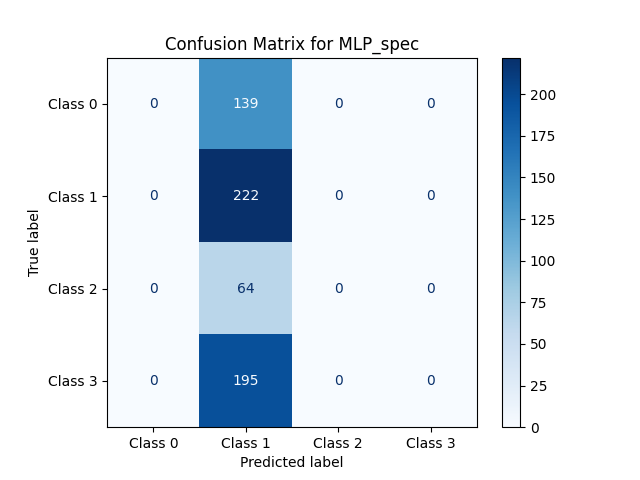
\includegraphics[width=\linewidth]{Figures/MLP_spec_confusion_mat.png} % Adjust path accordingly
        \caption{Confusion matrix for the DNN trained on the spectrogram data}
        \label{fig:MLP_spec_confusion_mat.png}
    \end{subfigure}
    \begin{subfigure}[b]{0.35\linewidth} % Another subfigure
        \centering
        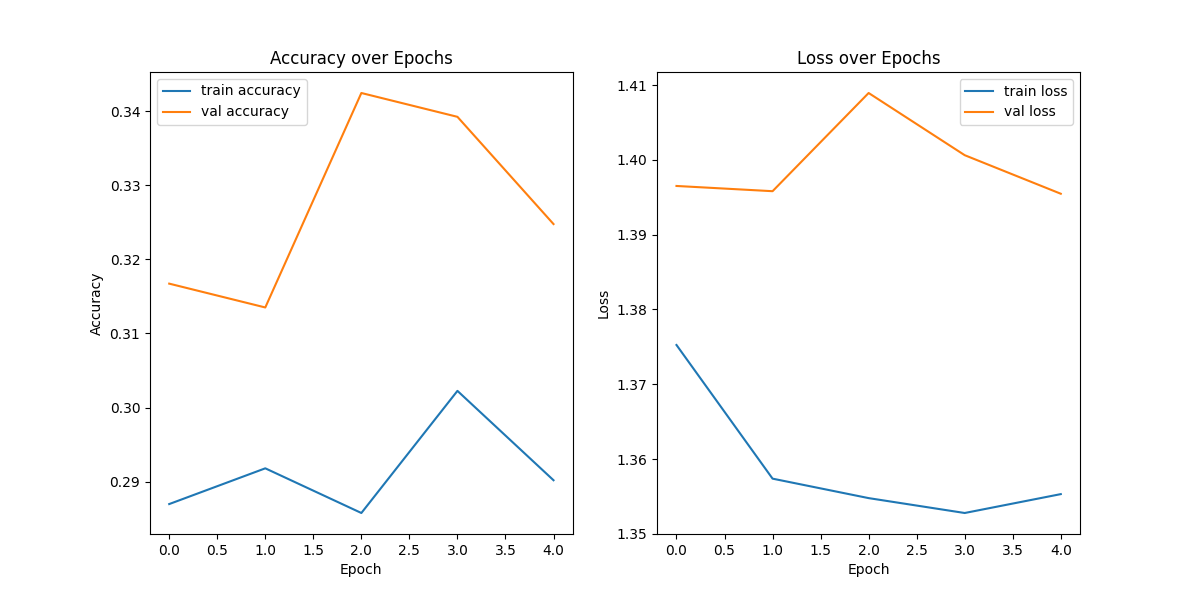
\includegraphics[width=\linewidth]{Figures/MLP_VT_loss_plot.png} % Adjust path accordingly
        \caption{Learning plots for the DNN trained on the voltage vs. time data}
        \label{fig:MLP_VT_loss_plot.png}
    \end{subfigure}
    \begin{subfigure}[b]{0.35\linewidth} % Another subfigure
        \centering
        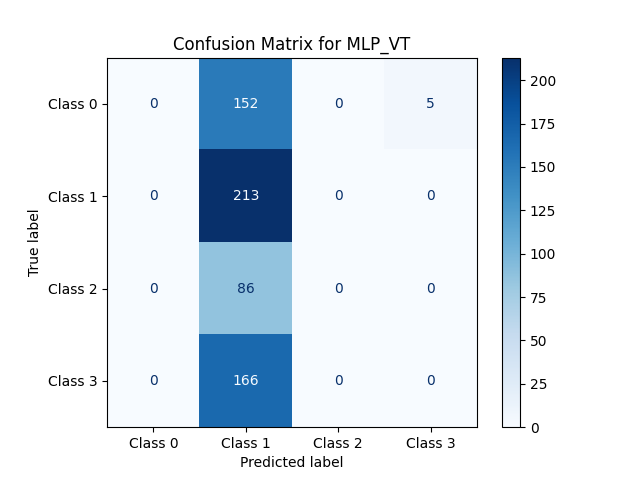
\includegraphics[width=\linewidth]{Figures/MLP_VT_confusion_mat.png} % Adjust path accordingly
        \caption{Confusion matrix for the DNN trained on the voltage vs. time data}
        \label{fig:MLP_VT_confusion_mat.png}
    \end{subfigure}
    \caption{Learning plots and confusion matrices from our 4 models}
    \label{fig:results}
\end{figure*}

\section{Discussion and Future Directions}
\subsection{Technical Issues}
\paragraph{Preprocessing}
One of the main differences between the preprocessing done in this study and in other successful studies was the use of Independent Component Analysis (ICA) instead of the Multiple Artifact Rejection Algorithm (MARA). MARA is a more advanced form of ICA that uses template matching to remove artifacts (Winkler, Haufe, \& Tangermann, 2011). ICA was selected instead for a simpler and more naturalistic analysis, but it is evident that MARA's added complexity yields higher accuracy (Marriott Haresign, 2021), so future attempts at this type of classification consider using MARA for artifact rejection.  

A separate issue that could have arisen in the preprocessing is the noisiness of the EEG data. Given that electroencephalograms are notoriously susceptible to environmental noise or physiological artifacts, it could be that the preprocessing steps taken were not enough to get rid of the noise in the system.

\paragraph{Network Construction and Data Compression}
Due to extensive time needed to construct the spectrogram, not much time was given towards constructing the neural networks, meaning they needed to be simplified considerably in order to avoid wasting additional time in training them. By simplifying the neural networks, their accuracy would decrease due to their weakened analytical properties. Moreover, the spectrogram was itself compressed significantly because the there were computing resource limitations, causing there to be less time bins and frequency bins in the spectrogram. This could negatively impact the models' ability to classify as the tainted spectrogram may have lost significant amounts of data necessary for feature extraction and ultimate classification.

\subsection{Conceptual Issues}


\subsubsection{Differences in Metrifying Emotion}

    The MUSIN-G dataset asked listeners to rate their enjoyment and familiarity of each song, using these variables as the behavioral response to the emotions felt by the music. However, this method is only one of many different ways to metrify emotion (Cui et.al., 2022). 
    
\paragraph{Physiological Stimuli}
Several of the more trusted methods of collecting emotional information stem from involuntary physiological responses to emotion-inducing stimuli; autonomic neural activity referenced by one's galvanic skin response, or emotional volatility measured by respiratory signals, are two examples of using spontaneous bodily cues (Zhang et.al., 2017; Das, Khasnobish, \& Tibarewala, 2016). That said, self-reporting emotional data has also been used frequently, albeit in different ways.

\paragraph{Difficulty in differentiating the spectrograms of different enjoyment-familiarity bins}
Observing the average spectrograms across different subjects keeping constant the channel and song, we find that it is difficult to differentiate between the spectrograms of different enjoyment-familiarity bins. 

To construct each spectrogram, we chose a song and EEG channel (in this case, channel 0 for all the spectrograms in Figure 8), found the subjects that gave HEHF ratings, found the subjects that had LELF ratings, and averaged the spectrogram data for each group from 10 to 20 seconds, which was well into when the stimulus started playing. 

For song 1, we can observe that the HEHF subjects had an average spectrogram that was hotter in the 25-35 Hz range than the LELF subjects. However, this pattern of difference does not continue for the other songs. For songs 9 and 12, it is difficult for the human eye to pick out very obvious differences between the HEHF and LELF data because both seem to be very sparse (mostly cold values).

Thus, while a more complex and computationally expensive model may be able to pick out the differences between the HEHF and LELF spectrograms since the human eye can't easily differentiate the 2 bins, it is also unlikely that our simple CNN or DNN (simple because of limited computational resources) used in this project would accomplish the classification task accurately for 4 classes, an even harder task.

\begin{figure*}
    \centering
    \begin{subfigure}[b]{0.45\linewidth} % Adjust the width of the subfigure, here it is 50% of the line width
        \centering
        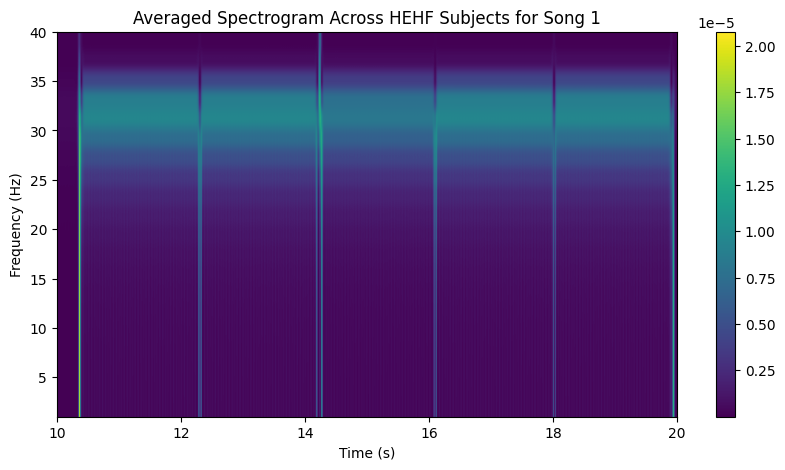
\includegraphics[width=\linewidth]{Figures/HEHF_1.png}
        \caption{}
        \label{fig:HEHF_1}
    \end{subfigure}%
    % add more subfigures here if you have more images
    \begin{subfigure}[b]{0.45\linewidth} % Another subfigure
        \centering
        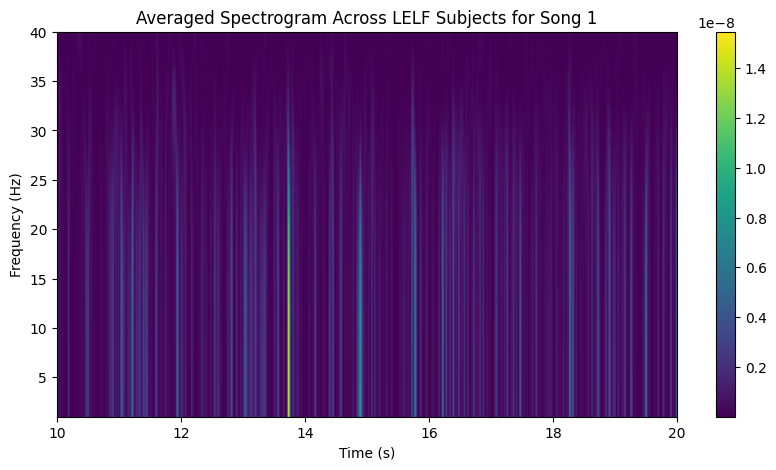
\includegraphics[width=\linewidth]{Figures/LELF_1.png} % Adjust path accordingly
        \caption{}
        \label{fig:LELF_1}
    \end{subfigure}
    \begin{subfigure}[b]{0.45\linewidth} % Another subfigure
        \centering
        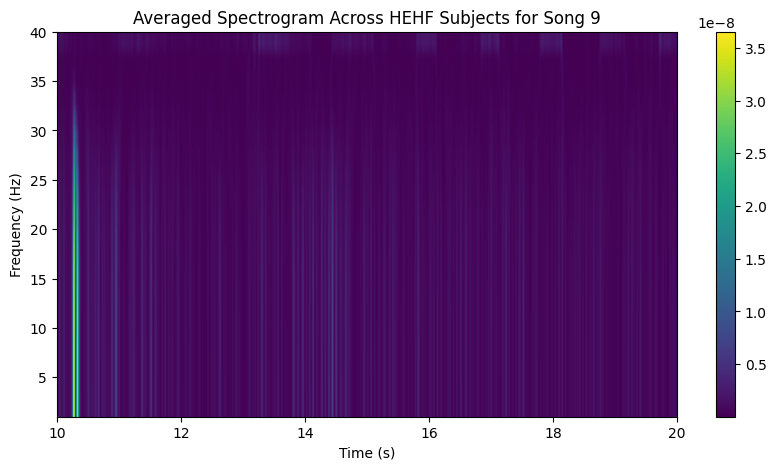
\includegraphics[width=\linewidth]{Figures/HEHF_9.png} % Adjust path accordingly
        \caption{}
        \label{fig:HEHF_9}
    \end{subfigure}
    \begin{subfigure}[b]{0.45\linewidth} % Another subfigure
        \centering
        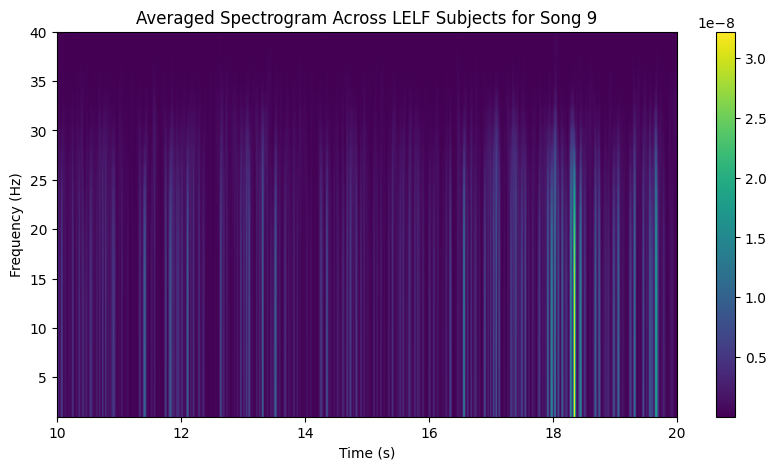
\includegraphics[width=\linewidth]{Figures/LELF_9.png} % Adjust path accordingly
        \caption{}
        \label{fig:LELF_9}
    \end{subfigure}
    \begin{subfigure}[b]{0.45\linewidth} % Another subfigure
        \centering
        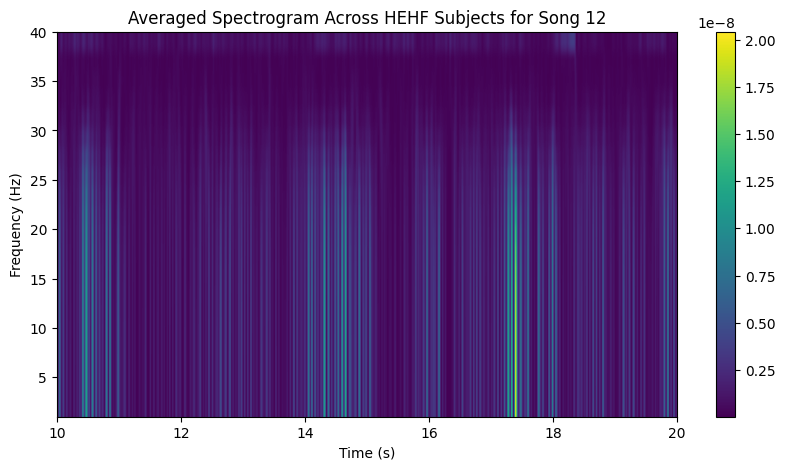
\includegraphics[width=\linewidth]{Figures/HEHF_12.png} % Adjust path accordingly
        \caption{}
        \label{fig:HEHF_12}
    \end{subfigure}
    \begin{subfigure}[b]{0.45\linewidth} % Another subfigure
        \centering
        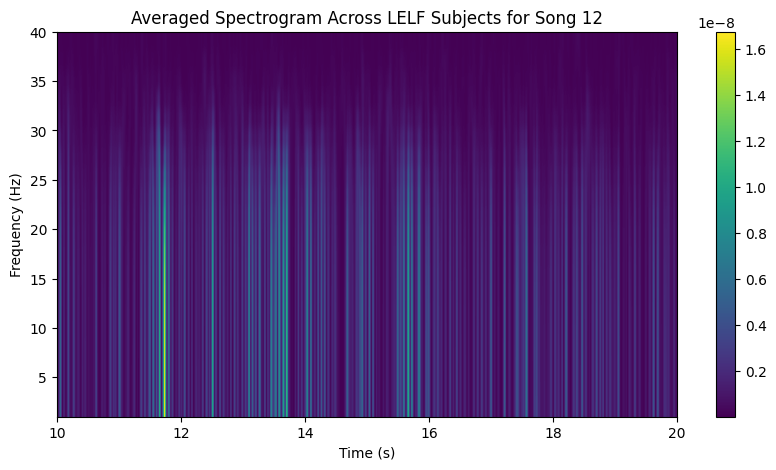
\includegraphics[width=\linewidth]{Figures/LELF_12.png} % Adjust path accordingly
        \caption{}
        \label{fig:LELF_12}
    \end{subfigure}
    \caption{Average spectrograms across different subjects keeping constant the channel and song. We choose to average across subjects who gave HEHF and LELF scores}
    \label{fig:avg_spec}
\end{figure*}

\paragraph{Defined Boolean Self-Reports}
Familiarity and enjoyment as metrics are themselves not unique to this study, but another study which used them effectively asked participants to choose either Yes or No to either metric, giving criteria such as "can predict what comes next" to further guide the participant to make the right choice (Pereira et.al., 2011). This is more effective than a number scale because the objective percent of familiarity is less intuitive than one's ability to justify why a song is familiar (and the same goes for enjoyment). 

\paragraph{Valence and Arousal}
The aforementioned metrics are not the most common. After being modernized in 1980 and validated in 1999, the Russell model for emotional affect-- defined by a 2D plane with valence and arousal as axes-- has become the most widely-used model for quantifying emotional information (Barrett \& Russell, 1999). \textbf{Valence} (the degree of an emotion's positivity or negativity) and \textbf{arousal} (the intensity of an emotion) allow for emotions to be distributed evenly across the plane, allowing it to be used either as a direct participant data-input or as a function to convert subjective emotional states (e.g. stressful, exciting, chill) into quantifiable emotional responses. Given that neural networks using these metrics appear to be more successful in the literature (Cui, Li, \& Touyama, 2023; Han, Chen, \& Ban, 2023; Qian et.al., 2022), it is a worthy future direction to consider using a dataset that employs these variables to improve the training and testing of our networks.

\subsubsection{Division of classes}

One of the clearest indications that training a model to predict the familiarity and enjoyment of a song excerpt would be challenging was that the range of those variables only went from 1 to 5, which decreased the divisibility of the data into equally sized categories. The parameters for what defined a high vs low familiarity or enjoyment (greater than vs. less than or equal to 2) do not accurately represent the distribution of the data as the majority of the respondents were relatively indifferent to the enjoyment of their music and generally very familiar with the music; this manifested in the dataset as a strong skew towards 3 in enjoyment and 4  or 5 in familiarity (see figure). Since 3 was mixed into ``high" with 4 and 5, the data's distribution was skewed such that falling into ``high" for both frequencies was significantly more likely. 

Using this information, we hypothesized that, if the networks were to predict a class unilaterally, it would be the High Enjoyment + High Frequency  class based purely on the behavioral data. However, noting that we applied random sampling upon feeding the data into the networks, this logic falls short as 3 out of the 4 network constructions unilaterally predicted High Enjoyment + Low Frequency, excluding the spectrogram-analyzing multi-layer perceptron which unilaterally predicted Low Enjoyment + Low Frequency. This leads us to conclude that the division of the behavioral data into classes, although faulty and improvable, was not the main cause of the reduced accuracy of the neural networks. In the future, assuming the same dataset is used, while creating a unique class for each combination of choices made by the listeners could resolve the issue of grouping concerns, it would significantly reduce the achievable accuracy of these neural networks in their simple form, so more investigation must be done to determine the ideal class size. 
- valence vs arousal
- others?

\subsubsection{Other Uses of the MUSIN-G Dataset}

While none of the current papers available online which have used the MUSIN-G dataset appear to have built neural networks in a similar manner, several authors of the paper have conducted additional experiments that could employ better ways to process and analyze the data. The closest study in similarity used Random Forest to analyze the differences between the listeners in the MUSIN-G dataset among 5 others, using the datasets themselves as the classes for which the algorithm was tested on (Pandey, Miyapuram, \& Lomas, 2022). This study's distinguishing method was that it aimed to predict the user's inherent brain signals in response to the music instead of using the self-reported behavioral results (thus accounting for implicit bias). Although this does not translate cleanly to our research questions, the direction towards predicting inherent traits, such as demographics, or physiological responses which are not self-reported, based on the EEG data merits consideration as a more feasible task given the type of data at hand. 
    One other key finding was that was that the quantity and localization of the electrodes in the MUSIN-G study could be optimized, such that by placing either 19 frontal electrodes or 18 central electrodes, the predictive accuracy of the RF model peaked at 70 and 80\%, respectively (Pandey, Miyapuram, \& Lomas, 2022). This implies that using electrode placement as a data input could yield promising results for classifying listeners using neural networks as well, thus making it a worthy future direction.

%------------------------------------------------

\phantomsection
\section*{Acknowledgments} % The \section*{} command stops section numbering

\paragraph{Matthew Vu:} All of Coding, Data Processing, Network Construction, Visualizations
\paragraph{Ricardo Marrero-Alattar:} All of Literature Review, Writing

\addcontentsline{toc}{section}{Acknowledgments}

\section*{References} % The \section*{} command stops section numbering

\addcontentsline{toc}{section}{References}% Adds this section to the table of contents


%----------------------------------------------------------------------------------------
%	REFERENCE LIST
%----------------------------------------------------------------------------------------

\begin{enumerate}
    \item  Alarcão, S. M., \& Fonseca, M. J. (2019). Emotions Recognition Using EEG Signals: A Survey. IEEE Transactions on Affective Computing, 10(3), 374-393. https://doi.org/10.1109/TAFFC.2017.2714671.
    \item Barrett, L. F., \& Russell, J. A. (1999). The Structure of Current Affect: Controversies and Emerging Consensus. Current Directions in Psychological Science, 8(1), 10-14. https://doi.org/10.1111/1467-8721.00003
    
    \item Carle, W. S. (2002). Comp.ai.neural-Nets FAQ, part 1 of 7: Introduction. faqs.org. http://www.faqs.org/faqs/ai-faq/neural-nets/part1/preamble.html 
    \item Chaddad, A., Wu, Y., Kateb, R., \& Bouridane, A. (2023). Electroencephalography Signal Processing: A Comprehensive Review and Analysis of Methods and Techniques. Sensors (Basel, Switzerland), 23(14), 6434. https://doi.org/10.3390/s23146434
    \item Cui, G., Li, X., \& Touyama, H. (2023). Emotion recognition based on group phase locking value using convolutional neural network. Scientific Reports, 13, 3769. https://doi.org/10.1038/s41598-023-30458-6
    \item Cui, X., Wu, Y., Wu, J., You, Z., Xiahou, J., \& Ouyang, M. (2022). A review: Music-emotion recognition and analysis based on EEG signals. Frontiers in Neuroinformatics, 16. https://doi.org/10.3389/fninf.2022.997282 
    \item   Das, P., Khasnobish, A., \& Tibarewala, D. (2016). Emotion recognition employing ECG and GSR signals as markers of ANS. In 2016 Conference on Advances in Signal Processing (CASP) (pp. 37-42). IEEE. 
    
    https://doi.org/10.1109/CASP.2016.7746134.

    \item de Boer, Kroese, D.P., Mannor, S. and Rubinstein, R.Y. (2005). A tutorial on the cross-entropy method. Annals of Operations Research 134 (1), 19–67.
    \item Ding, Y., Robinson, N., Tong, C., Zeng, Q., \& Guan, C. (2023). LGGNet: Learning From Local-Global-Graph Representations for Brain–Computer Interface. IEEE Transactions on Neural Networks and Learning Systems. https://doi.org/10.1109/TNNLS.2023.3236635

    \item Ghodousi, M., Pousson, J. E., Voicikas, A., Bernhofs, V., Pipinis, E., Tarailis, P., Burmistrova, L., Lin, Y. P., \& Griškova-Bulanova, I. (2022). EEG Connectivity during Active Emotional Musical Performance. Sensors (Basel, Switzerland), 22(11), 4064. 
    
    https://doi.org/10.3390/s22114064
    \item Han, X., Chen, F., \& Ban, J. (2023). Music Emotion Recognition Based on a Neural Network with an Inception-GRU Residual Structure. Electronics, 12, 978.
    
    https://doi.org/10.3390/electronics12040978
    \item He, N., \& Ferguson, S. (2020). Multi-view Neural Networks for Raw Audio-based Music Emotion Recognition. In 2020 IEEE International Symposium on Multimedia (ISM) (pp. 168-172). Naples, Italy. doi: 10.1109/ISM.2020.00037.

    \item Jadon, A. K., \& Kumar, S. (2023). A Comparative Study of CNNs and DNNs for Emotion Detection from text using TF-IDF. In International Conference on Advances in Computation, Communication and Information Technology (ICAICCIT) (pp. 1329-1334). Faridabad, India. 
    
    https://doi.org/10.1109/ICAICCIT60255.2023.10465903.

    \item Jia X. (2022). Music Emotion Classification Method Based on Deep Learning and Improved Attention Mechanism. Computational intelligence and neuroscience, 2022, 5181899. https://doi.org/10.1155/2022/5181899

    \item Kamala, A., \& Hassani, H. (2022). Kurdish music genre recognition using a CNN and DNN. ASEC 2022.
    
    https://doi.org/10.3390/asec2022-13803 

    \item Koelstra, S., Muhl, C., Soleymani, M., Jong-Seok Lee, Yazdani, A., Ebrahimi, T., Pun, T., Nijholt, A., \& Patras, I. (2012). DEAP: A database for emotion analysis; using physiological signals. IEEE Transactions on Affective Computing, 3(1), 18–31. https://doi.org/10.1109/t-affc.2011.15 

    \item Leo, C. (2024, April 9). The math behind Adam Optimizer. Medium. https://towardsdatascience.com/the-math-behind-adam-optimizer-c41407efe59b 

    \item Madison, G., \& Schiölde, G. (2017). Repeated Listening Increases the Liking for Music Regardless of Its Complexity: Implications for the Appreciation and Aesthetics of Music. Frontiers in neuroscience, 11, 147. https://doi.org/10.3389/fnins.2017.00147
    \item Marriott Haresign, I., Phillips, E., Whitehorn, M., Noreika, V., Jones, E. J. H., Leong, V., \& Wass, S. V. (2021). Automatic classification of ICA components from infant EEG using Mara. Developmental Cognitive Neuroscience, 52, 101024. 
    
    https://doi.org/10.1016/j.dcn.2021.101024 
    \item Miyapuram, K. P., Ahmad, N., Pandey, P., \& Lomas, J. D. (2022). Electroencephalography (EEG) dataset during naturalistic music listening comprising different genres with familiarity and enjoyment ratings. Data in brief, 45, 108663. https://doi.org/10.1016/j.dib.2022.108663
    \item Miyapuram, K. P., Pandey, P., Ahmad, N., Shiraguppi, B. R., Sharma, E., Lawhatre, P., Sonawane, D., \& Lomas, D. (2022). Music Listening- Genre EEG dataset (MUSIN-G). OpenNeuro. [Dataset]. 
    
    https://doi.org/10.18112/openneuro.ds003774.v1.0.2.

    \item MNE Developers. (n.d.). Documentation overview. MNE 1.7.0 documentation. 
    
    https://mne.tools/stable/documentation/index.html 
    
    \item Newman, A. J. (n.d.). MNE-Python. Neural Data Science in Python. https://neuraldatascience.io/7-eeg/mne\_python.html

    \item Pandey, P., Bedmutha, P. S., Miyapuram, K. P., \& Lomas, D. (2023). Stronger correlation of music features with brain signals predicts increased levels of enjoyment. In 2023 IEEE Applied Sensing Conference (APSCON) (pp. 1-3). Bengaluru, India. 
    
    https://doi.org/10.1109/APSCON56343.2023.10101229.
    \item Pandey, P., Miyapuram, K. P., \& Lomas, D. (2022, August 22). Non-Linear Features of $\beta$ Brain Rhythms Predict Listener-Specific Neural Signature in Naturalistic Music Listening. TechRxiv. 
    
    https://doi.org/10.36227/techrxiv.16571411.v1
    
    \item Pereira, C. S., Teixeira, J., Figueiredo, P., Xavier, J., Castro, S. L., \& Brattico, E. (2011). Music and emotions in the brain: familiarity matters. PloS one, 6(11), e27241. https://doi.org/10.1371/journal.pone.0027241

    \item Picard, R. W. (2003). Affective computing: Challenges. International Journal of Human-Computer Studies, 59(1–2), 55–64. https://doi.org/10.1016/s1071-5819(03)00052-1 
    \item Qian, W., Tan, J., Jiang, Y., \& Tian, Y. (2022). Deep learning with convolutional neural networks for EEG-based music emotion decoding and visualization. Brain-Apparatus Communication: A Journal of Bacomics, 1(1), 38–49. 
    
    https://doi.org/10.1080/27706710.2022.2075241
    \item Shen, F., Peng, Y., Kong, W., \& Dai, G. (2021). Multi-Scale Frequency Bands Ensemble Learning for EEG-Based Emotion Recognition. Sensors, 21(4), 1262. https://doi.org/10.3390/s21041262.
    \item Vuilleumier, P., and Trost, W. (2015). Music and emotions: from enchantment to entrainment. Ann. N. Y. Acad. Sci. 1337, 212–222. doi: 10.1111/nyas.12676
    \item Winkler, I., Haufe, S., \& Tangermann, M. (2011). Automatic classification of artifactual ICA-components for artifact removal in EEG signals. Behavioral and Brain Functions, 7
    \item Zhang, Q., Chen, X., Zhan, Q., Yang, T., \& Xia, S. (2017). Respiration-based emotion recognition with deep learning. Computers in Industry, 92, 84-90.
    
    https://doi.org/10.1016/j.compind.2017.04.005.
    \item Zhou, T. H., Liang, W., Liu, H., Wang, L., Ryu, K. H., \& Nam, K. W. (2023). EEG emotion recognition applied to the effect analysis of music on emotion changes in psychological healthcare. International Journal of Environmental Research and Public Health, 20(1), 378. https://doi.org/10.3390/ijerph20010378

    
    
\end{enumerate}


















































%----------------------------------------------------------------------------------------

\end{document}